\subsection{Performance estimation}
\label{sec:performance}

In this section, we describe the first phase of Elo-MMR. For notational convenience, we assume all probability expressions to be conditioned on the \textbf{prior context} $P_{i,< t}$, and omit the subscript $t$.

Our prior belief on each player's skill $S_i$ implies a prior distribution on $P_i$. Let's denote its probability density function (pdf) by
\begin{equation}
\label{eq:perf-prior} 
f_i(p) := \Pr(P_i = p) = \int \pi_i(s) \Pr(P_i = p \mid S_i=s) \,\mathrm{d}s,
\end{equation}
where $\pi_i(s)$ was defined in \Cref{eq:pi-s}. Let
\[F_i(p) := \Pr(P_i\le p) = \int_{-\infty}^p f_i(x) \,\dx,\]
be the corresponding cumulative distribution function (cdf). For the purpose of analysis, we'll also define the following ``loss'', ``draw'', and ``victory'' functions:
\begin{align*}
l_i(p) &:= \ddp\ln(1-F_i(p)) = \frac{-f_i(p)}{1 - F_i(p)},
\\d_i(p) &:= \ddp\ln f_i(p) = \frac{f'_i(p)}{f_i(p)},
\\v_i(p) &:= \ddp\ln F_i(p) = \frac{f_i(p)}{F_i(p)}.
\end{align*}

Evidently, $l_i(p) < 0 < v_i(p)$. Now we define what it means for the deviation $P_i - S_i$ to be log-concave.
\begin{definition}
\label{def:log-concave}
An absolutely continuous random variable on a convex domain is \textbf{log-concave} if its probability density function $f$ is positive on its domain and satisfies
\[f(\theta x + (1-\theta) y) > f(x)^\theta f(y)^{1-\theta},\;\forall\theta\in(0,1),x\neq y.\]
\end{definition}

Log-concave distributions appear widely, and include the Gaussian and logistic distributions used in Glicko, TrueSkill, and many others. We'll see inductively that our prior $\pi_i$ is log-concave at every round. Since log-concave densities are closed under convolution~\cite{concave}, the independent sum $P_i=S_i+(P_i-S_i)$ is also log-concave. Log-concavity is made very convenient by the following lemma, proved in the extended version of this paper:
\begin{lemma}
\label{lem:decrease}
If $f_i$ is continuously differentiable and log-concave, then the functions $l_i,d_i,v_i$ are continuous, strictly decreasing, and
\[l_i(p) < d_i(p) < v_i(p) \text{ for all }p.\]
\end{lemma}

For the remainder of this section, we fix the analysis with respect to some player $i$. As argued in \Cref{sec:bayes_model}, $P_i$ concentrates very narrowly in the posterior. Hence, we can estimate $P_i$ by its MAP, choosing $p$ so as to maximize:
\[\Pr(P_i=p\mid E^L_i,E^W_i) \propto f_i(p) \Pr(E^L_i,E^W_i\mid P_i=p).\]

Define $j\succ i$, $j\prec i$, $j\sim i$ as shorthand for $j\in E^L_i$, $j\in E^W_i$, $j\in \mathcal P\setminus (E^L_i\cup E^W_i)$ (that is, $P_j>P_i$, $P_j<P_i$, $P_j=P_i$), respectively. The following theorem yields our MAP estimate:
\begin{theorem}
\label{thm:uniq-max}
Suppose that for all $j$, $f_j$ is continuously differentiable and log-concave. Then the unique maximizer of $\Pr(P_i=p\mid E^L_i,E^W_i)$ is given by the unique zero of
\[Q_i(p) := \sum_{j \succ i} l_j(p) + \sum_{j \sim i} d_j(p) + \sum_{j \prec i} v_j(p).\]
\end{theorem}
The proof appears in the extended version of this paper. Intuitively, we're saying that the performance is the balance point between appropriately weighted wins, draws, and losses. Let's look at two specializations of our general model, to serve as running examples in this paper.

\paragraph{Gaussian performance model}
If both $S_j$ and $P_j-S_j$ are assumed to be Gaussian with known means and variances, then their independent sum $P_j$ will also be a known Gaussian. It is analytic and log-concave, so \Cref{thm:uniq-max} applies.

We substitute the well-known Gaussian pdf and cdf for $f_j$ and $F_j$, respectively. A simple binary search, or faster numerical techniques such as the Illinois algorithm or Newton's method, can be employed to solve for the unique zero of $Q_i$.

\begin{figure}
    \centering
    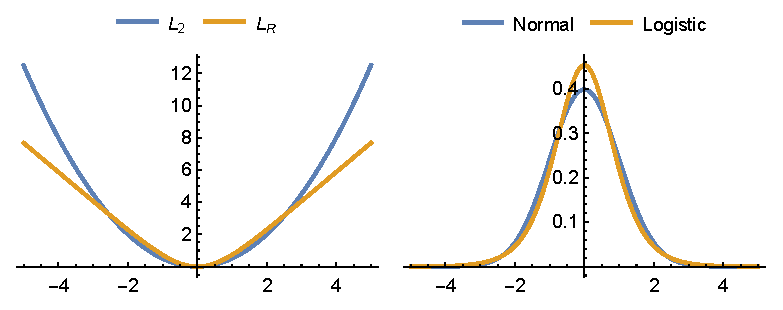
\includegraphics[width=1.05\columnwidth]{images/l2-lr-plot.eps}
    \caption{$L_2$ versus $L_R$ for typical values (left). Gaussian versus logistic probability density functions (right).}
    \label{fig:l2-lr-plot}
\end{figure}

\paragraph{Logistic performance model}
Now we assume the performance deviation $P_j-S_j$ has a logistic distribution with mean 0 and variance $\beta^2$. In general, the rating system administrator is free to set $\beta$ differently for each contest. Since shorter contests tend to be more variable, one reasonable choice might be to make $1/\beta^2$ proportional to the contest duration.

Given the mean and variance of the skill prior, the independent sum $P_j = S_j + (P_j-S_j)$ would have the same mean, and a variance that's increased by $\beta^2$. Unfortunately, we'll see that the logistic performance model implies a form of skill prior from which it's tough to extract a mean and variance. Even if we could, the sum does not yield a simple distribution.

For experienced players, we expect $S_j$ to contribute much less variance than $P_j-S_j$; thus, in our heuristic approximation, we take $P_j$ to have the same form of distribution as the latter. That is, we take $P_j$ to be logistic, centered at the prior rating $\mu^\pi_j = \argmax \pi_j$, with variance $\delta_j^2 = \sigma_j^2 + \beta^2$, where $\sigma_j$ will be given by \Cref{eq:variance}. This distribution is analytic and log-concave, so the same methods based on \Cref{thm:uniq-max} apply. 
Define the scale parameter $\bar\delta_j := \frac{\sqrt{3}}{\pi} \delta_j$. A logistic distribution with variance $\delta_j^2$ has cdf and pdf:
\begin{align*}
F_j(x) &= \frac { 1 } { 1 + e^{-(x-\mu^\pi_j)/\bar\delta_j} }
= \frac 12 \left(1 + \tanh\frac{x-\mu^\pi_j}{2\bar\delta_j} \right),
\\f_j(x) &= \frac { e^{(x-\mu^\pi_j)/\bar\delta_j} } { \bar\delta_j\left( 1 + e^{(x-\mu^\pi_j)/\bar\delta_j} \right)^2}
= \frac { 1 } { 4\bar\delta_j} \sech^2\frac{x-\mu^\pi_j}{2\bar\delta_j}.
\end{align*}

The logistic distribution satisfies two very convenient relations:
\begin{align*}
F'_j(x) = f_j(x) &= F_j(x) (1 - F_j(x)) / \bar\delta_j,
\\f'_j(x) &= f_j(x) (1 - 2F_j(x)) / \bar\delta_j,
\end{align*}
from which it follows that
\[d_j(p)
= \frac{1 - 2F_j(p)}{\bar\delta}
= \frac{-F_j(p)}{\bar\delta} + \frac{1 - F_j(p)}{\bar\delta}
= l_j(p) + v_j(p).\]

In other words, a tie counts as the sum of a win and a loss. This can be compared to the approach (used in Elo, Glicko, BAR, Topcoder, and Codeforces) of treating each tie as half a win plus half a loss.\footnote{Elo-MMR, too, can be modified to split ties into half win plus half loss. It's easy to check that \Cref{lem:decrease} still holds if $d_j(p)$ is replaced by
$w_l l_j(p) + w_v v_j(p)$
for some $w_l,w_v\in [0,1]$ with $|w_l-w_v|<1$.
In particular, we can set $w_l=w_v=0.5$. The results in \Cref{sec:properties} won't be altered by this change.}

Finally, putting everything together:
\[Q_i(p) = \sum_{j \succeq i} l_j(p) + \sum_{j \preceq i} v_j(p)
= \sum_{j \succeq i} \frac{-F_j(p)}{\bar\delta_j} + \sum_{j \preceq i} \frac{1 - F_j(p)}{\bar\delta_j}.\]
Our estimate for $P_i$ is the zero of this expression. The terms on the right correspond to probabilities of winning and losing against each player $j$, weighted by $1/\bar\delta_j$. Accordingly, we can interpret $\sum_{j\in \cP} (1-F_j(p))/\bar\delta_j$ as a weighted expected rank of a player whose performance is $p$. Similar to the performance computations in Codeforces and Topcoder, $P_i$ can thus be viewed as the performance level at which one's expected rank would equal $i$'s actual rank.

